% 第三章 Hopfion 稳定性研究
\chapter{Hopfion 稳定性研究}

本章研究 Hopfion 在两种磁性体系中的稳定条件：含体积型 DMI 的铁磁体系（以 FeGe 为代表）和竞争交换铁磁体系。本章通过微磁学模拟，确定各体系中 Hopfion 稳定存在的必要条件和参数范围。


\section{DMI 铁磁体系中的 Hopfion 稳定性}

\subsection{FeGe 材料参数与模型设置}

本文选取手性磁体 FeGe 作为研究对象，其材料参数如\cref{tab:fege-params}所示。FeGe 的螺旋周期 $\lambda = 4\pi A_{\text{ex}} / |D_{\text{bulk}}| \approx \SI{70}{nm}$，这一特征长度决定了模型的空间尺度。

\begin{table}[htbp]
  \centering
  \caption{FeGe 材料参数}
  \label{tab:fege-params}
  \begin{tabular}{lll}
    \toprule
    参数 & 符号 & 数值 \\
    \midrule
    饱和磁化强度 & $M_s$ & $\SI{384e3}{A/m}$ \\
    交换刚度 & $A_{\text{ex}}$ & $\SI{8.78e-12}{J/m}$ \\
    体积型 DMI 常数 & $D_{\text{bulk}}$ & $\SI{1.58e-3}{J/m^2}$ \\
    螺旋周期 & $\lambda$ & $\SI{70}{nm}$ \\
    \bottomrule
  \end{tabular}
\end{table}

模型采用圆柱形几何，直径 $d = \SI{210}{nm} = 3\lambda$，高度 $h = \SI{70}{nm} = \lambda$。网格尺寸为 $\SI{1}{nm} \times \SI{1}{nm} \times \SI{1}{nm}$，满足交换长度分辨要求。

\subsection{初始态构造：Sutcliffe 解析解}

Hopfion 的初始磁化构型采用 Sutcliffe 提出的解析解\cite{sutcliffe2018hopfions}进行构造。该解基于有理映射近似，能够给出拓扑荷 $Q_H = 1$ 的 Hopfion 磁化分布。初始态通过 Python 脚本计算并输出为 OVF 格式文件，供 Mumax3 加载。

在 Hopfion 核心区域，$m_z$ 从中心的 $-1$（反向磁化管）过渡到外围的 $+1$（均匀背景），中间形成环面状的旋转过渡区。

\subsection{稳定性的三个必要条件}

通过对比实验，本文确定了 FeGe 体系中 Hopfion 稳定存在的三个必要条件：

\textbf{条件一：解析初始态。} 使用随机或简单环形（torus）初始态均无法收敛到 Hopfion 亚稳态。只有基于 Sutcliffe 解析解构造的初始态，其磁化分布才处于 Hopfion 能量盆地的吸引域内。

\textbf{条件二：边界层冻结。} 模型顶部和底部边界层的磁化固定为 $\mathbf{m} = \hat{z}$（通过 Mumax3 的 \texttt{frozenspins} 功能实现）。若不冻结边界层，DMI 倾向于在边界处形成螺旋态，破坏 Hopfion 所需的均匀背景。

\textbf{条件三：退磁场效应。} 必须启用退磁场计算（\texttt{EnableDemag = true}）。退磁场提供了额外的形状各向异性，有助于维持 $m_z = +1$ 的背景磁化，从而稳定 Hopfion 结构。

\cref{tab:fege-conditions}总结了各条件组合的仿真结果。

\begin{table}[htbp]
  \centering
  \caption{FeGe 体系中 Hopfion 稳定条件的对比实验}
  \label{tab:fege-conditions}
  \begin{tabular}{cccc}
    \toprule
    解析初始态 & 边界冻结 & 退磁场 & 结果 \\
    \midrule
    \checkmark & \checkmark & \checkmark & 稳定（2 ns） \\
    \checkmark & \checkmark & $\times$   & 螺旋态 \\
    \checkmark & $\times$   & \checkmark & 螺旋态 \\
    $\times$   & \checkmark & \checkmark & 不收敛 \\
    \bottomrule
  \end{tabular}
\end{table}

\subsection{弛豫与演化结果}

在满足三个必要条件后，首先以 $\alpha = 0.5$ 的高阻尼进行弛豫（Relax），使初始态收敛到局部能量极小值。随后以 $\alpha = 0.02$ 进行 \SI{2}{ns} 的时间演化。结果表明 Hopfion 保持稳定，$\langle m_z \rangle = 0.376$，核心半径约 \SI{50}{nm}。

\cref{fig:fege-stable}展示了弛豫后 Hopfion 的稳态结构。左图为 $z = 0$ 中平面的 $m_z$ 分布，清晰显示了中心反向磁化区域（$m_z = -1$，深蓝色）和环形过渡区；中图为 $y = 0$ 截面，展示了 Hopfion 沿 $z$ 轴方向的管状核心结构；右图为面内磁化分量分布，呈现出 Bloch 型的旋转特征。

\begin{figure}[htbp]
  \centering
  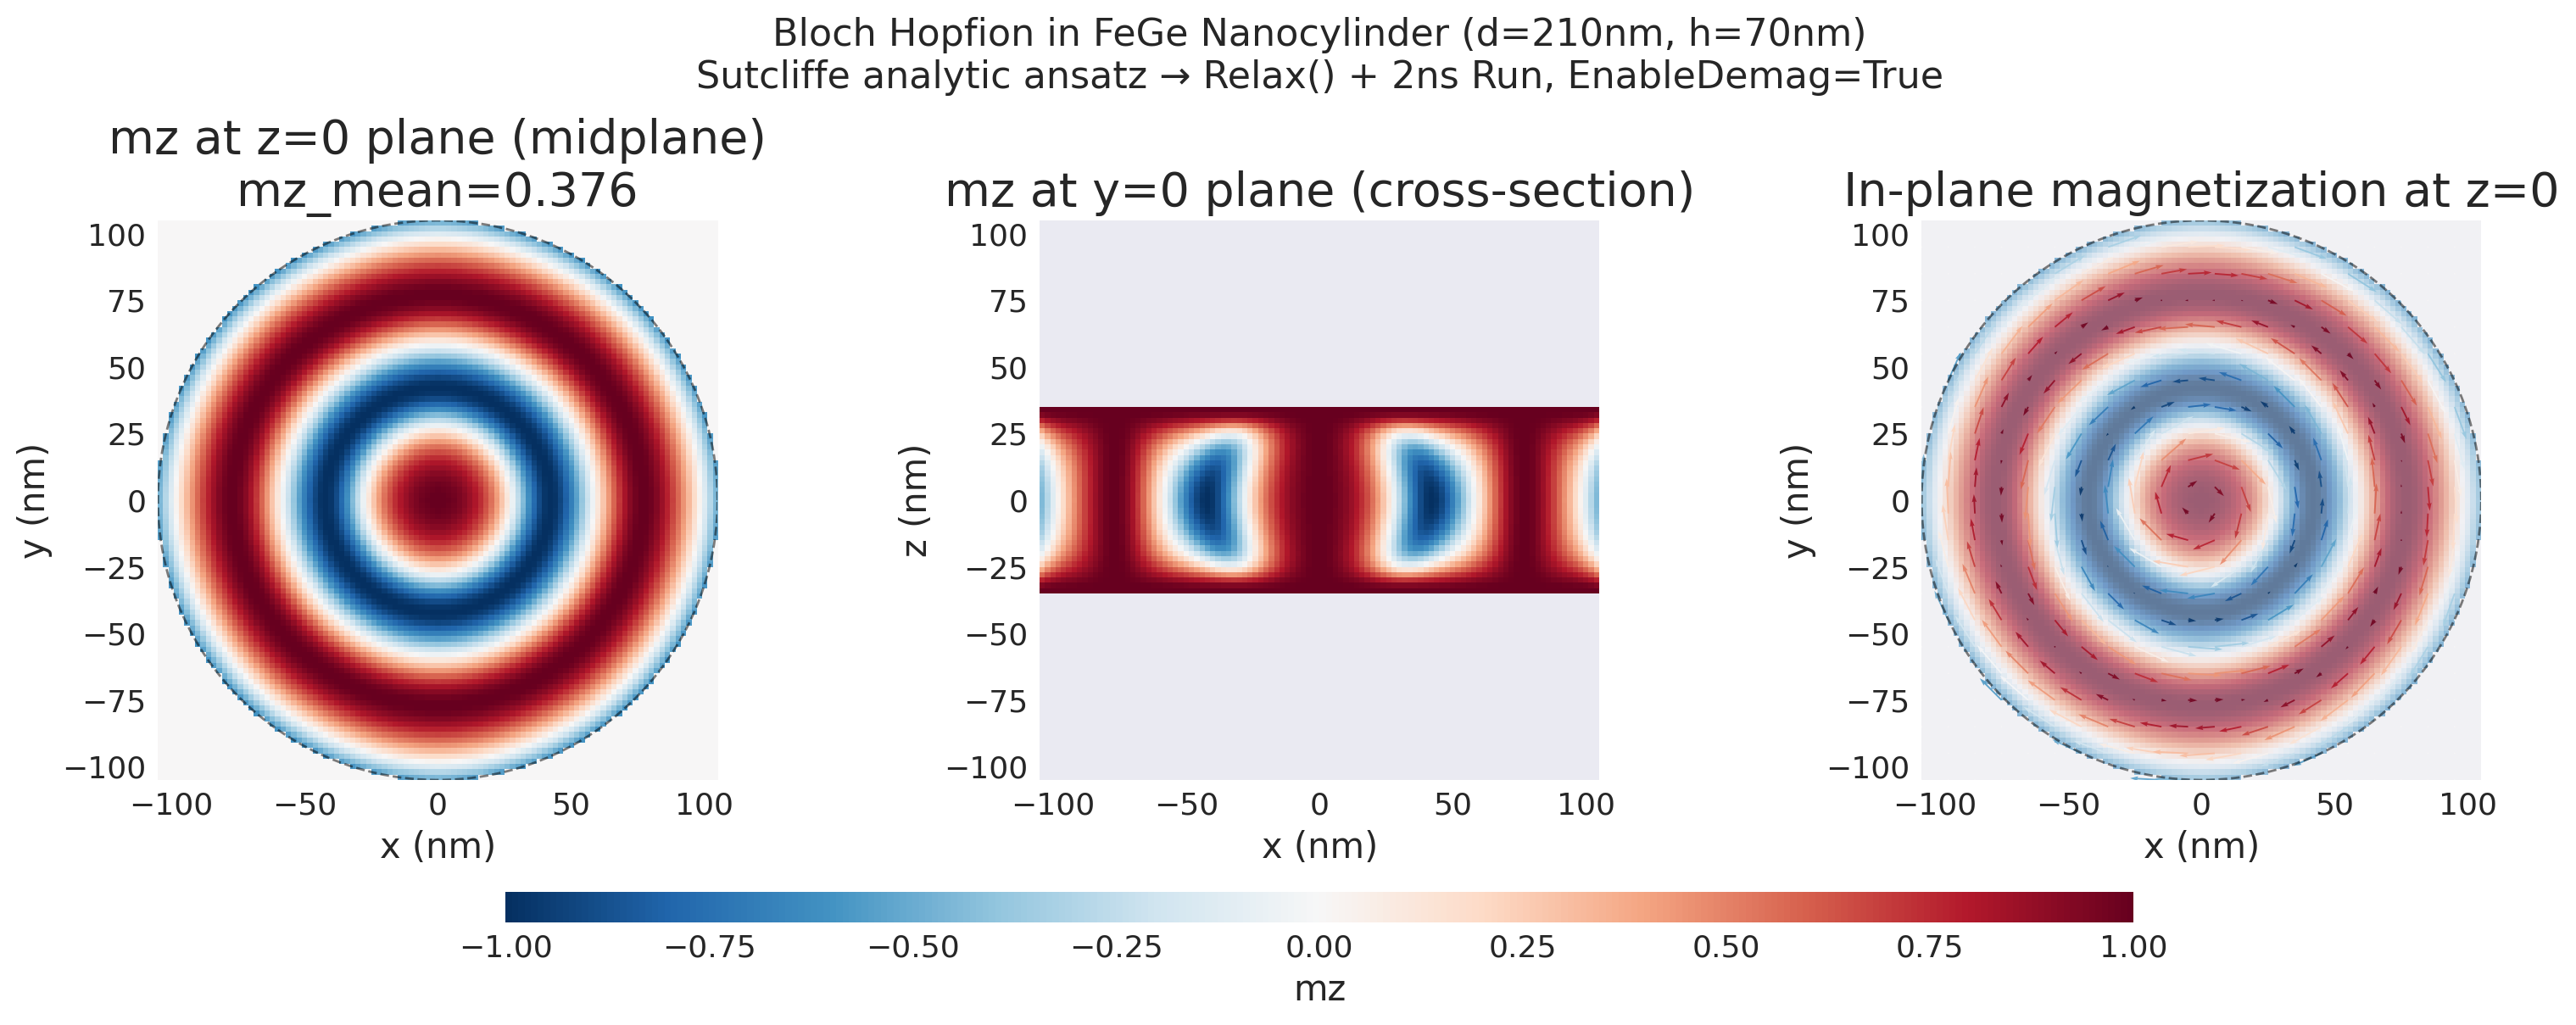
\includegraphics[width=0.95\textwidth]{figures/fig3-1_fege_hopfion_stable.png}
  \caption{FeGe 体系中 Bloch 型 Hopfion 经弛豫和 \SI{2}{ns} 时间演化后的稳态结构。左：$z = 0$ 中平面 $m_z$ 分布（$\langle m_z \rangle = 0.376$）；中：$y = 0$ 截面；右：面内磁化分量}
  \label{fig:fege-stable}
\end{figure}


\section{竞争交换铁磁体系中的 Hopfion 稳定性}

\subsection{模型设置}

竞争交换铁磁体系的灵感来源于 Sallermann 等人的理论工作\cite{sallermann2023stability}。Lobanov 和 Uzdin 进一步研究了该体系中 Hopfion 的寿命、坍塌路径和逃逸机制\cite{lobanov2023lifetime}。模型参数如\cref{tab:frustrated-params}所示。

\begin{table}[htbp]
  \centering
  \caption{竞争交换铁磁体系参数}
  \label{tab:frustrated-params}
  \begin{tabular}{lll}
    \toprule
    参数 & 符号 & 数值 \\
    \midrule
    饱和磁化强度 & $M_s$ & $\SI{1.5e5}{A/m}$ \\
    最近邻交换刚度 & $A_{\text{ex}}$ ($J_1$) & $\SI{5e-12}{J/m}$ \\
    次近邻交换 & $J_2$ & $-0.164 \, J_1$ \\
    第四近邻交换 & $J_4$ & $-0.082 \, J_1$ \\
    模型尺寸 & — & $\SI{50}{nm} \times \SI{50}{nm} \times \SI{50}{nm}$ \\
    网格 & — & $100 \times 100 \times 100$ \\
    格点间距 & — & $\SI{0.5}{nm}$ \\
    边界条件 & — & 三维周期性边界 \\
    \bottomrule
  \end{tabular}
\end{table}

与 DMI 体系不同，该体系无 DMI、无磁晶各向异性、无退磁场，Hopfion 的稳定完全依赖竞争交换相互作用。采用三维周期性边界条件（PBC）模拟无限大体块。

\subsection{漂移稳定性分析}

Hopfion 在均匀磁化背景中是否会自发漂移，是评估其器件可用性的关键指标。为此，本文在控制变量条件下（统一 $\alpha = 0.2$、$K_{u1} = 0$、相同尺寸初始态 $R = \SI{3}{nm}$, $r = \SI{2}{nm}$、运行时间 \SI{2}{ns}），设计了四组对比实验，比较了不同背景磁化方向（$m_z$、$m_x$、$m_y$）和 Hopfion 轴向（$z$ 轴、$x$ 轴、$y$ 轴）的组合。

\cref{tab:drift-results}总结了漂移实验结果。\textbf{四组配置的行为完全一致}：Hopfion 质心在前 $\sim\SI{1}{ns}$ 沿其环面轴向发生 $\approx \SI{4.75}{nm}$ 的一次性位移后完全钉扎，横向位移始终为零。这表明背景磁化方向对 Hopfion 的漂移行为没有影响。

\begin{table}[htbp]
  \centering
  \caption{控制变量漂移实验结果汇总（统一参数：$\alpha = 0.2$, $K_{u1} = 0$, $R_0 = \SI{3}{nm}$, $r_0 = \SI{2}{nm}$）}
  \label{tab:drift-results}
  \begin{tabular}{ccccc}
    \toprule
    配置 & 背景方向 & Hopfion 轴向 & 轴向位移 & 横向位移 \\
    \midrule
    bg=$m_z$, axis=$z$ & $m_z = +1$ & $z$ & $+\SI{4.75}{nm}$ ($z$) & $\SI{0}{nm}$ \\
    bg=$m_z$, axis=$x$ & $m_z = +1$ & $x$ & $+\SI{4.75}{nm}$ ($x$) & $\SI{0}{nm}$ \\
    bg=$m_y$, axis=$y$ & $m_y = +1$ & $y$ & $+\SI{4.75}{nm}$ ($y$) & $\SI{0}{nm}$ \\
    bg=$m_x$, axis=$x$ & $m_x = +1$ & $x$ & $+\SI{4.75}{nm}$ ($x$) & $\SI{0}{nm}$ \\
    \bottomrule
  \end{tabular}
\end{table}

观测到的 \SI{4.75}{nm} 轴向位移来自初始态的格点弛豫。连续解析构造的 Hopfion ansatz 放到离散格点上后，质心会从初始位置迁移到最近的格点势能极小值。这个弛豫过程在 $\sim\SI{1}{ns}$ 内完成，之后 Hopfion 被格点势牢固钉扎。弛豫方向严格沿 Hopfion 环面轴向，因为轴向的格点势势垒较浅，而环面平面内的钉扎势较深。

\cref{fig:drift-comparison}展示了四组实验的总漂移距离对比。所有曲线在误差范围内完全重合，进一步确认了背景磁化方向的无关性。选取 $m_x = +1$ 背景进行 \SI{10}{ns} 长时间验证（\cref{fig:drift-10ns}），Hopfion 在完成初始弛豫后的 \SI{9}{ns} 内质心完全静止，$y$、$z$ 方向全程零漂移，长时稳定性得以确认。

\begin{figure}[htbp]
  \centering
  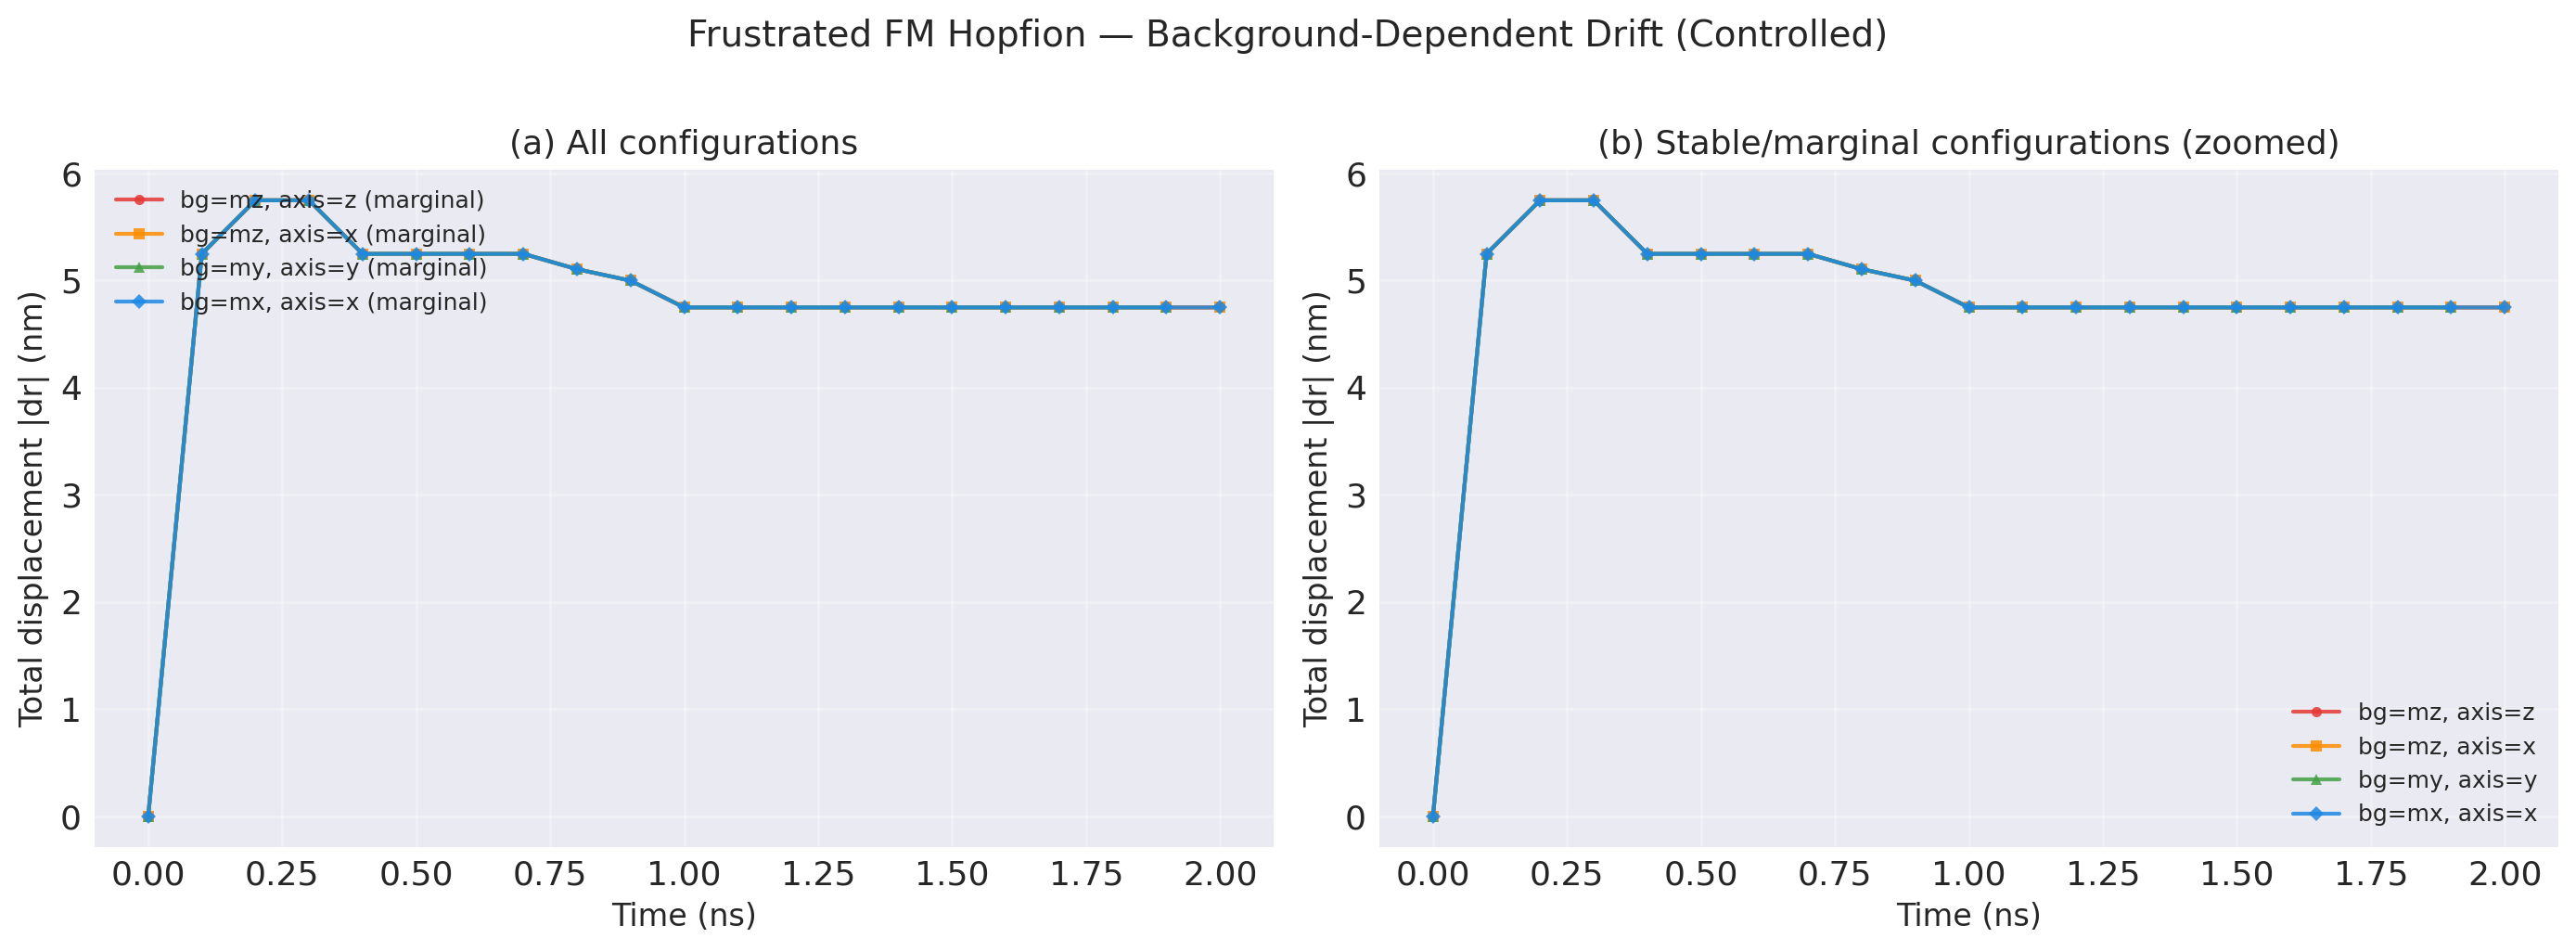
\includegraphics[width=0.95\textwidth]{figures/fig3-4_drift_comparison.png}
  \caption{四组配置的总漂移距离 $|\Delta r|$ 随时间的演化。所有曲线完全重合：前 $\sim\SI{1}{ns}$ 内质心因格点弛豫沿轴向位移 $\approx\SI{4.75}{nm}$，此后完全钉扎。背景磁化方向（$m_z$、$m_x$、$m_y$）对漂移行为无影响}
  \label{fig:drift-comparison}
\end{figure}

\begin{figure}[htbp]
  \centering
  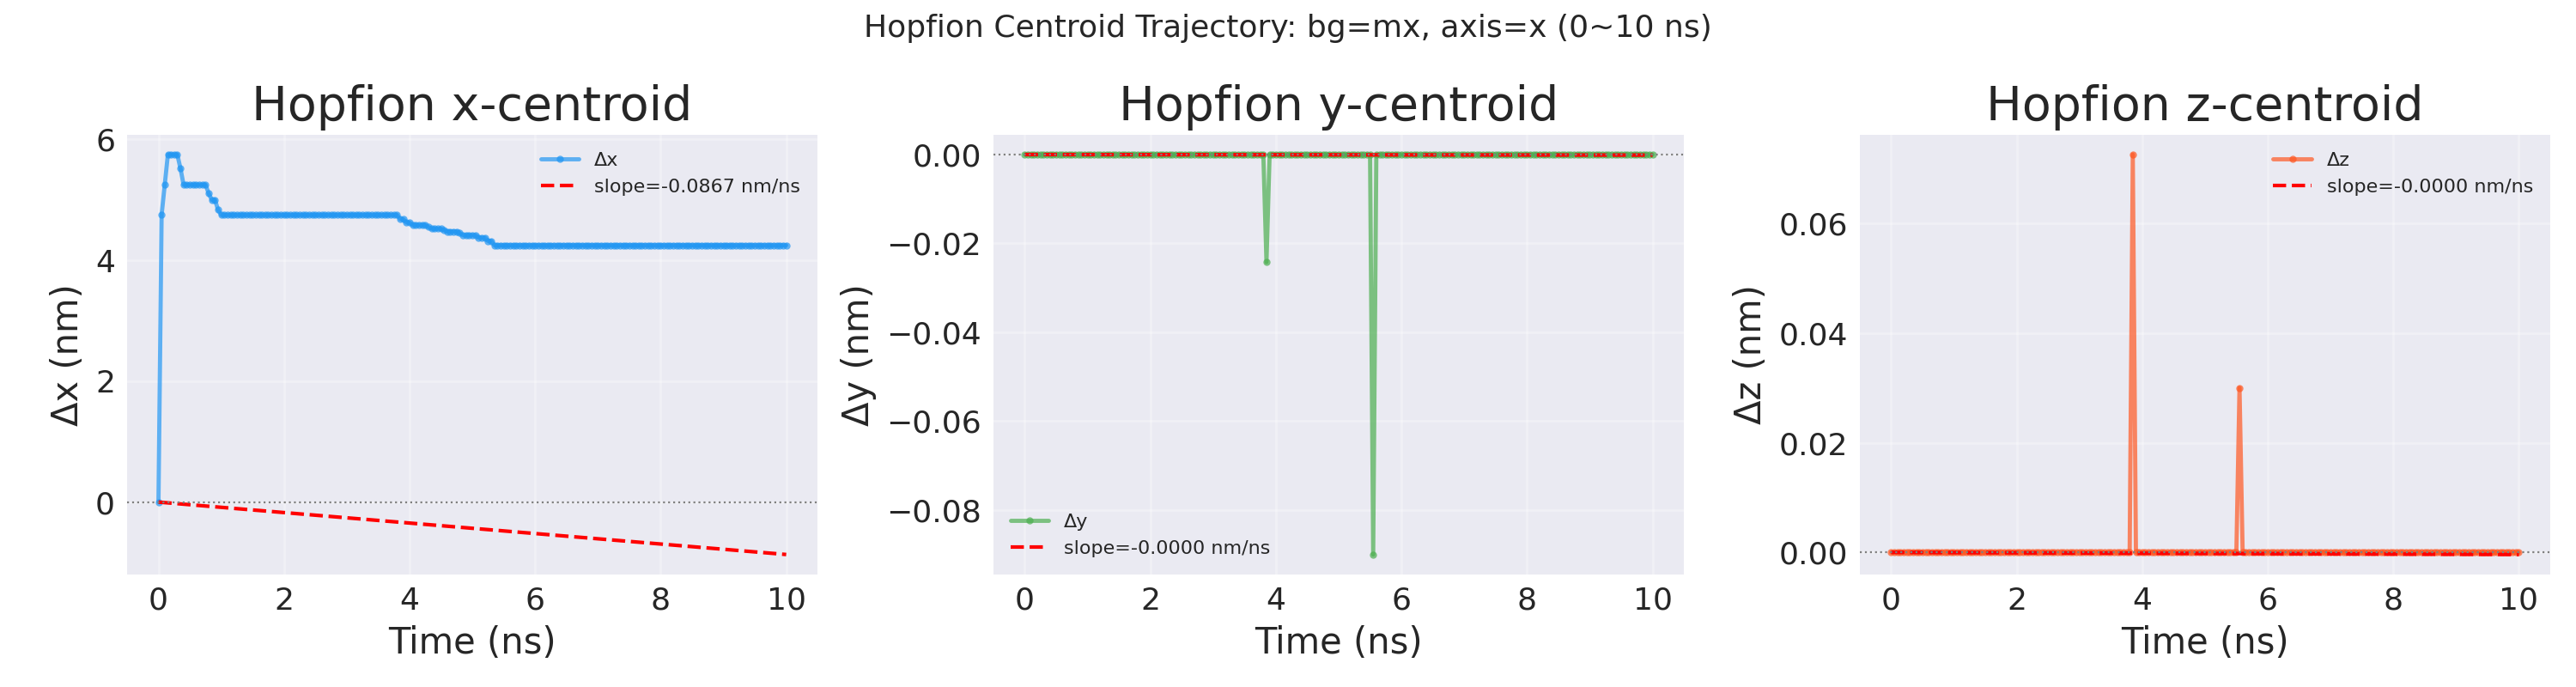
\includegraphics[width=0.95\textwidth]{figures/fig3-4_drift_trajectory_10ns.png}
  \caption{$m_x = +1$ 背景下 Hopfion 的 \SI{10}{ns} 质心轨迹。$x$ 方向（Hopfion 轴向）在前 \SI{1}{ns} 内发生 $\approx\SI{4.75}{nm}$ 一次性格点弛豫后完全钉扎；$y$、$z$ 方向全程零漂移}
  \label{fig:drift-10ns}
\end{figure}

\subsection{居中稳态验证}

在上述漂移稳定性分析中，所有 $m_z = +1$ 背景下的 Hopfion 都发生了 $z$ 方向漂移（详见 \cref{tab:drift-results}），弛豫后质心偏离了其初始设定位置。这给后续的自旋波仿真带来了问题：偏移的 Hopfion 靠近吸收边界层，自旋波还没到达 Hopfion 核心就被衰减了。

为了解决这个问题，本文采用了\textbf{周期性平移}方法。利用三维周期性边界条件的平移不变性，本文将弛豫后的磁化构型沿 $z$ 轴整体平移，使 Hopfion 质心回到盒子几何中心 $(\SI{25}{nm}, \SI{25}{nm}, \SI{25}{nm})$。平移操作通过 NumPy 的 \texttt{np.roll} 函数实现，磁化分布保持不变，只改变其在周期性盒子中的位置。

平移后的构型需要重新验证稳定性。选取三组代表性配置（$K_{u1} = 0$、$\SI{10e3}{}$、$\SI{50e3}{J/m^3}$），在 $\alpha = 0.2$、PBC 条件下各运行 \SI{1}{ns}，监控 Hopfion 质心位置和核心细胞数（$m_z < 0$ 的格点数）。判定标准：$z$ 方向漂移 $|\Delta z| < \SI{2}{nm}$。

\cref{tab:centered-stability}汇总了验证结果。三组配置全部通过稳态判定，最大漂移仅 $\SI{0.70}{nm}$（$K_{u1} = 0$），$K_{u1} = \SI{10e3}{J/m^3}$ 的漂移更是低至 $\SI{0.019}{nm}$，表现出极高的位置稳定性。

\begin{table}[htbp]
  \centering
  \caption{居中 Hopfion 的 \SI{1}{ns} 稳态验证结果}
  \label{tab:centered-stability}
  \begin{tabular}{ccccc}
    \toprule
    $K_{u1}$ (J/m$^3$) & $z_0$ (nm) & $z_{\text{final}}$ (nm) & $\Delta z$ (nm) & 核心细胞数 \\
    \midrule
    0     & 28.44 & 29.15 & $+0.70$ & 1984 $\to$ 2128 \\
    10000 & 25.07 & 25.05 & $-0.019$ & 920 $\to$ 908 \\
    50000 & 25.13 & 25.19 & $+0.062$ & 388 $\to$ 404 \\
    \bottomrule
  \end{tabular}
\end{table}

\cref{fig:centered-z-drift}展示了三组配置的 $z$ 方向漂移随时间的演化。$K_{u1} = 0$ 表现出约 $\SI{1}{nm}$ 振幅的呼吸模式振荡，但长时间平均漂移可控；$K_{u1} = \SI{10e3}{}$ 和 $\SI{50e3}{J/m^3}$ 则几乎完全静止。\cref{fig:centered-core-count}展示了核心细胞数的时间演化：$K_{u1} = \SI{10e3}{}$ 和 $\SI{50e3}{J/m^3}$ 的核心尺寸高度稳定，$K_{u1} = 0$ 的振荡与其 $z$ 方向的呼吸模式一致。

综合各项指标，$K_{u1} = \SI{10e3}{J/m^3}$ 的居中 Hopfion 在位置稳定性和结构保持方面均为最优，因此已消除了初始的漂移不确定性。在此基础上，本文进一步研究各向异性参数对处于居中稳态下的 Hopfion 的影响。

\begin{figure}[htbp]
  \centering
  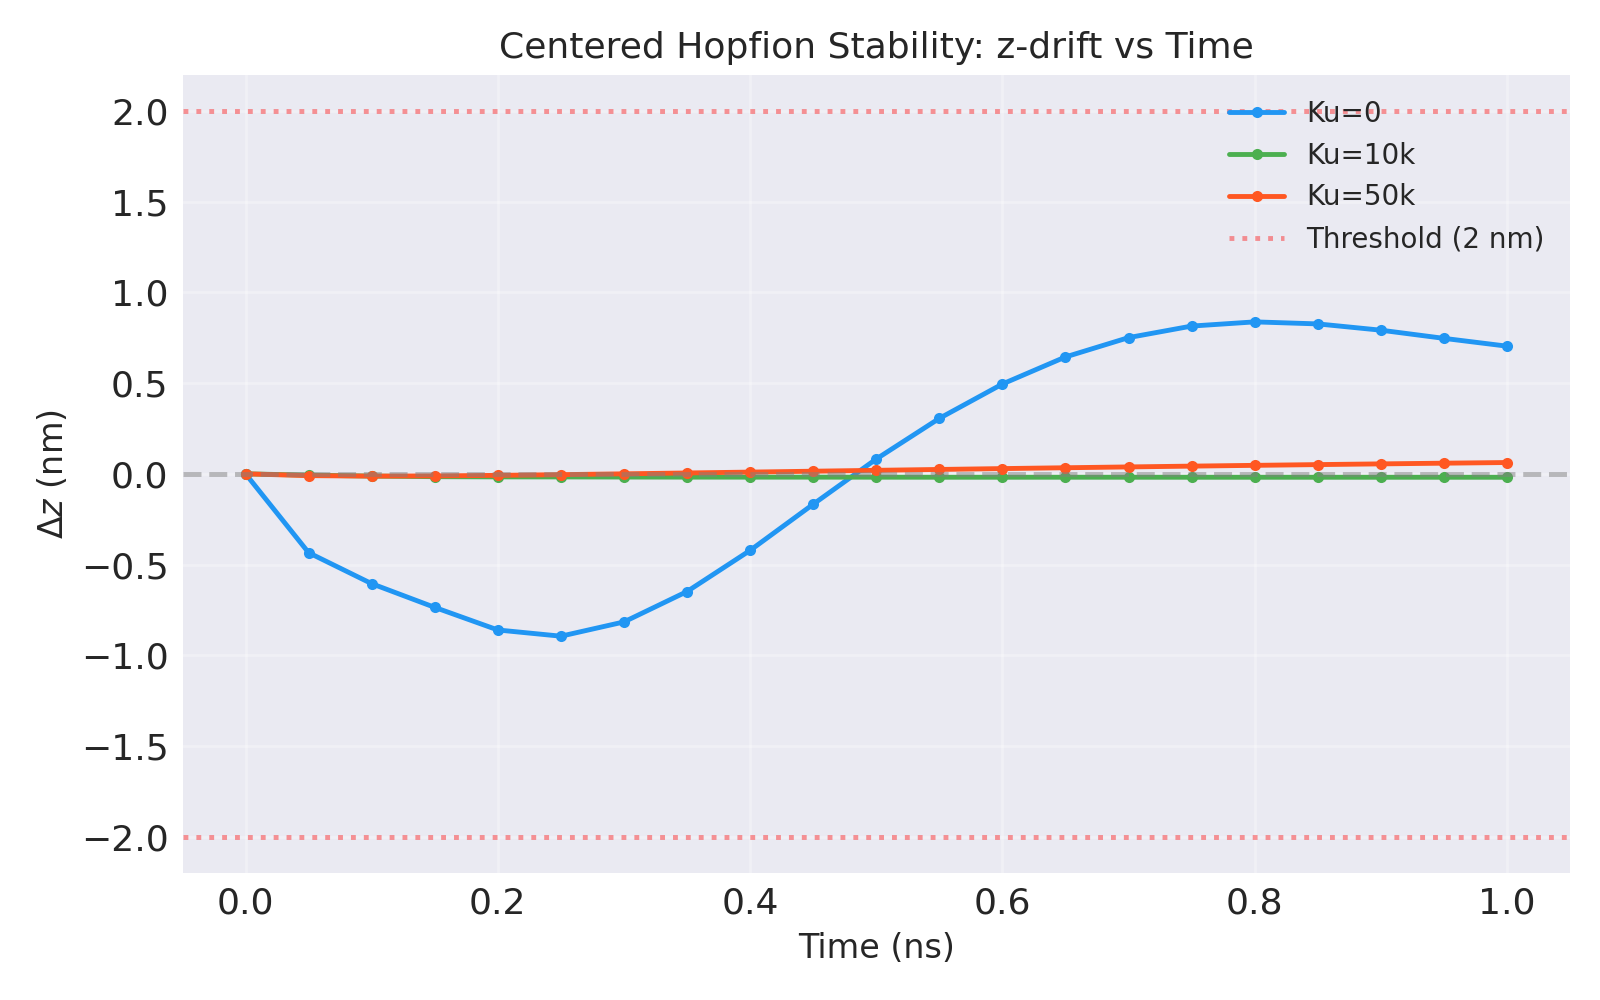
\includegraphics[width=0.85\textwidth]{figures/fig3-8_centered_z_drift.png}
  \caption{居中 Hopfion 的 $z$ 方向漂移随时间演化。虚线标记 $\pm\SI{2}{nm}$ 判定阈值。$K_{u1} = 0$ 表现为呼吸模式振荡，$K_{u1} = \SI{10e3}{}$ 和 $\SI{50e3}{J/m^3}$ 几乎无漂移}
  \label{fig:centered-z-drift}
\end{figure}

\begin{figure}[htbp]
  \centering
  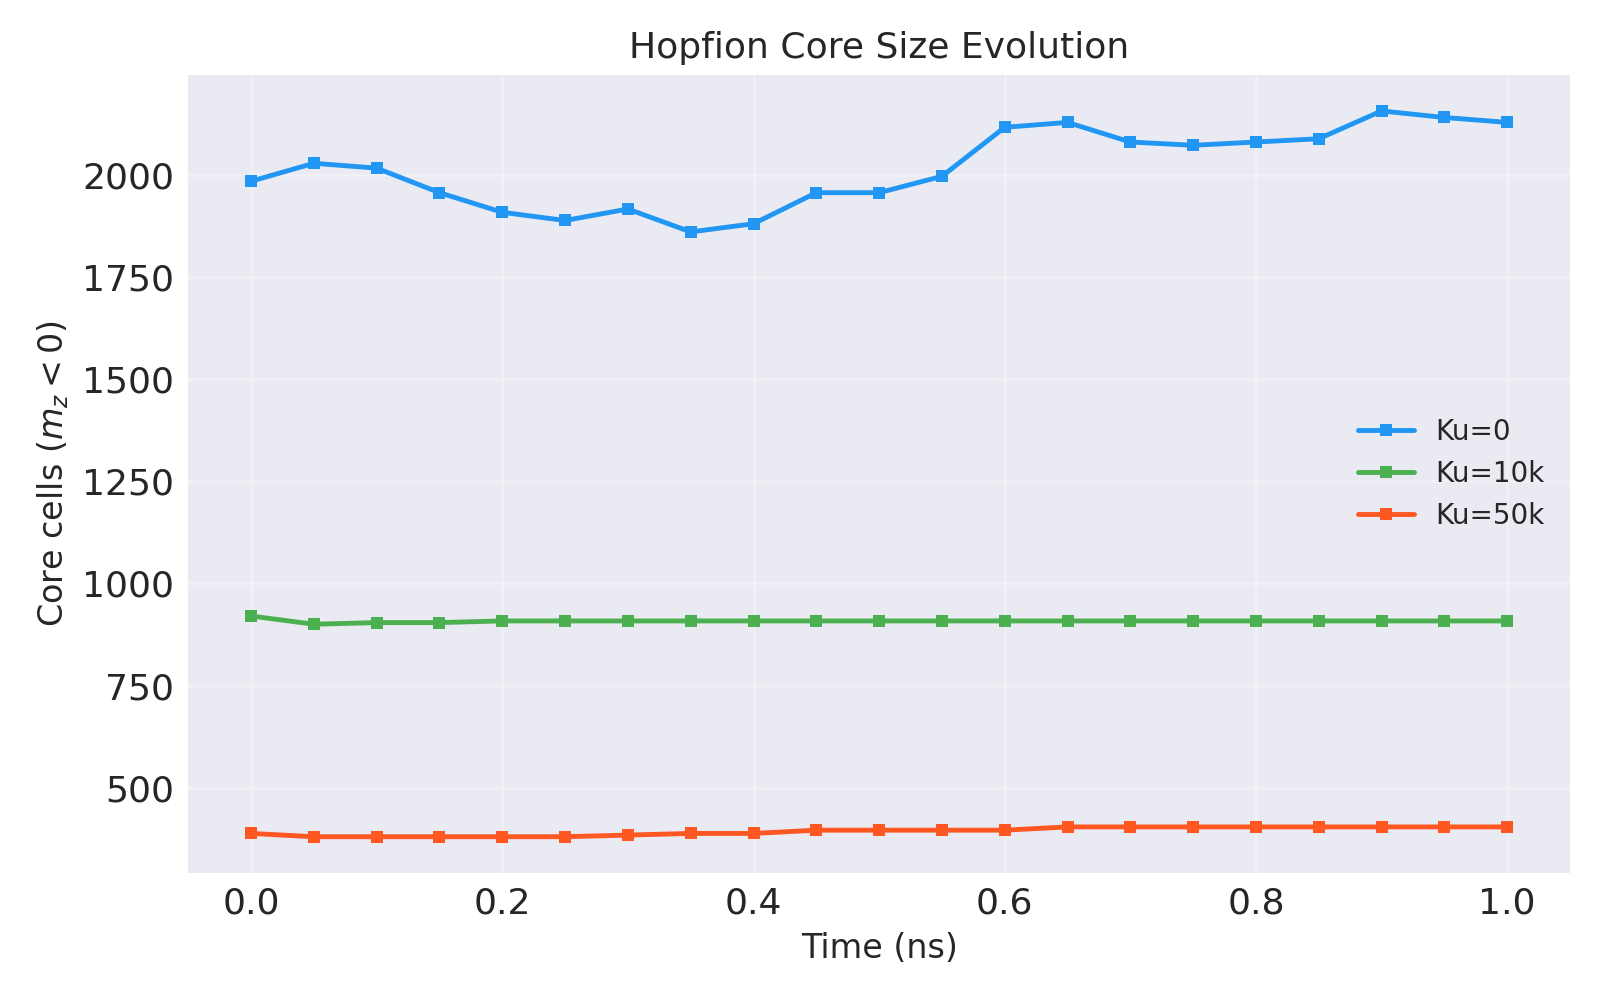
\includegraphics[width=0.85\textwidth]{figures/fig3-9_centered_core_count.png}
  \caption{Hopfion 核心细胞数（$m_z < 0$）随时间演化。各向异性越强，核心越小但越稳定}
  \label{fig:centered-core-count}
\end{figure}


\subsection{各向异性对稳定性的影响}

在竞争交换体系中引入单轴磁晶各向异性 $K_{u1}$（沿 Hopfion 轴向），研究其对已证实具有居中稳定性的 Hopfion 结构的影响。扫描范围为 $K_{u1} = 0 \sim \SI{75e3}{J/m^3}$，其中 $\SIrange{50e3}{58e3}{J/m^3}$ 区间以 $\SI{1e3}{J/m^3}$ 间距进行了细化扫描。以弛豫后的 $R = \SI{8}{nm}$、$r = \SI{4}{nm}$ Hopfion 为初始态，每组在 $\alpha = 0.2$ 下运行 \SI{1}{ns}。

\cref{fig:anisotropy-time}展示了不同 $K_{u1}$ 下 Hopfion 环面半径 $R$ 和管径 $r$ 随时间的演化。所有构型从相同初始尺寸出发，在约 \SI{0.6}{ns} 内收敛到各自的平衡态。$K_{u1}$ 越大，平衡后的 $R$ 和 $r$ 越小，反映了各向异性对 Hopfion 结构的压缩效应。

\cref{tab:ku-sweep-large}汇总了各组 $K_{u1}$ 在 $t = \SI{1}{ns}$ 时的尺寸参数。$K_{u1} = \SI{52e3}{J/m^3}$ 时 Hopfion 仍然存活，核心体素数从初始的 20344 缩减至 376，对应管径约 $\SI{1.2}{nm}$（$\sim 2.4$ 个格点）。$K_{u1} = \SI{55e3}{J/m^3}$ 时核心体素数归零，Hopfion 完全坍塌为均匀态。$K_{u1} = \SI{75e3}{J/m^3}$ 时，仿真在 \SI{0.37}{ns} 处即因数值不稳定而中断。

\begin{table}[htbp]
  \centering
  \caption{不同 $K_{u1}$ 下 Hopfion 弛豫 \SI{1}{ns} 后的尺寸参数}
  \label{tab:ku-sweep-large}
  \begin{tabular}{cccc}
    \toprule
    $K_{u1}$ (J/m$^3$) & $R$ (nm) & $r$ (nm) & 状态 \\
    \midrule
    0     & 2.63 & 2.22 & 稳定 \\
    5000  & 2.35 & 1.85 & 稳定 \\
    10000 & 2.17 & 1.64 & 稳定 \\
    20000 & 1.82 & 1.54 & 稳定 \\
    30000 & 1.82 & 1.38 & 稳定 \\
    50000 & 1.56 & 1.24 & 稳定 \\
    52000 & 1.50 & 1.20 & 稳定（临界） \\
    55000 & —    & —    & 坍缩 \\
    75000 & —    & —    & 坍缩 \\
    \bottomrule
  \end{tabular}
\end{table}

由此本文确定了\textbf{临界各向异性阈值}：
\begin{equation}
  K_{u1,c} \in (\num{52e3}, \, \num{55e3}) \, \si{J/m^3}
  \label{eq:ku-critical}
\end{equation}

这一临界行为可以从能量竞争的角度理解。Hopfion 管径 $r$ 由三方面能量的平衡决定：（1）交换能 $\sim A_{\text{ex}}/r^2$，倾向于增大管径；（2）竞争交换（$J_2$、$J_4$）提供的拓扑约束，将 $r$ 锁定在固有吸引子尺寸附近；（3）各向异性能 $\sim K_{u1} r^2 L$（$L$ 为管长），倾向于缩小反向磁化体积，从而压缩管径。

当 $K_{u1}$ 较小时，拓扑约束与交换能的竞争占主导，$r$ 在吸引子附近稳定。随 $K_{u1}$ 增大，各向异性的收缩力不断增强。在 $K_{u1,c}$ 处，收缩力超过了拓扑抵抗，管径被压缩到格点分辨率（$\sim \SI{0.5}{nm}$）的量级，拓扑结构在离散网格上无法维持，Hopfion 就会坍缩。这一结果与 Metlov 关于螺旋磁体中 Hopfion 椭圆稳定性的理论分析定性一致\cite{metlov2025elliptical}。\cref{fig:anisotropy-summary}展示了 $R$ 和 $r$ 随 $K_{u1}$ 单调递减的趋势和临界区域的位置。

\begin{figure}[htbp]
  \centering
  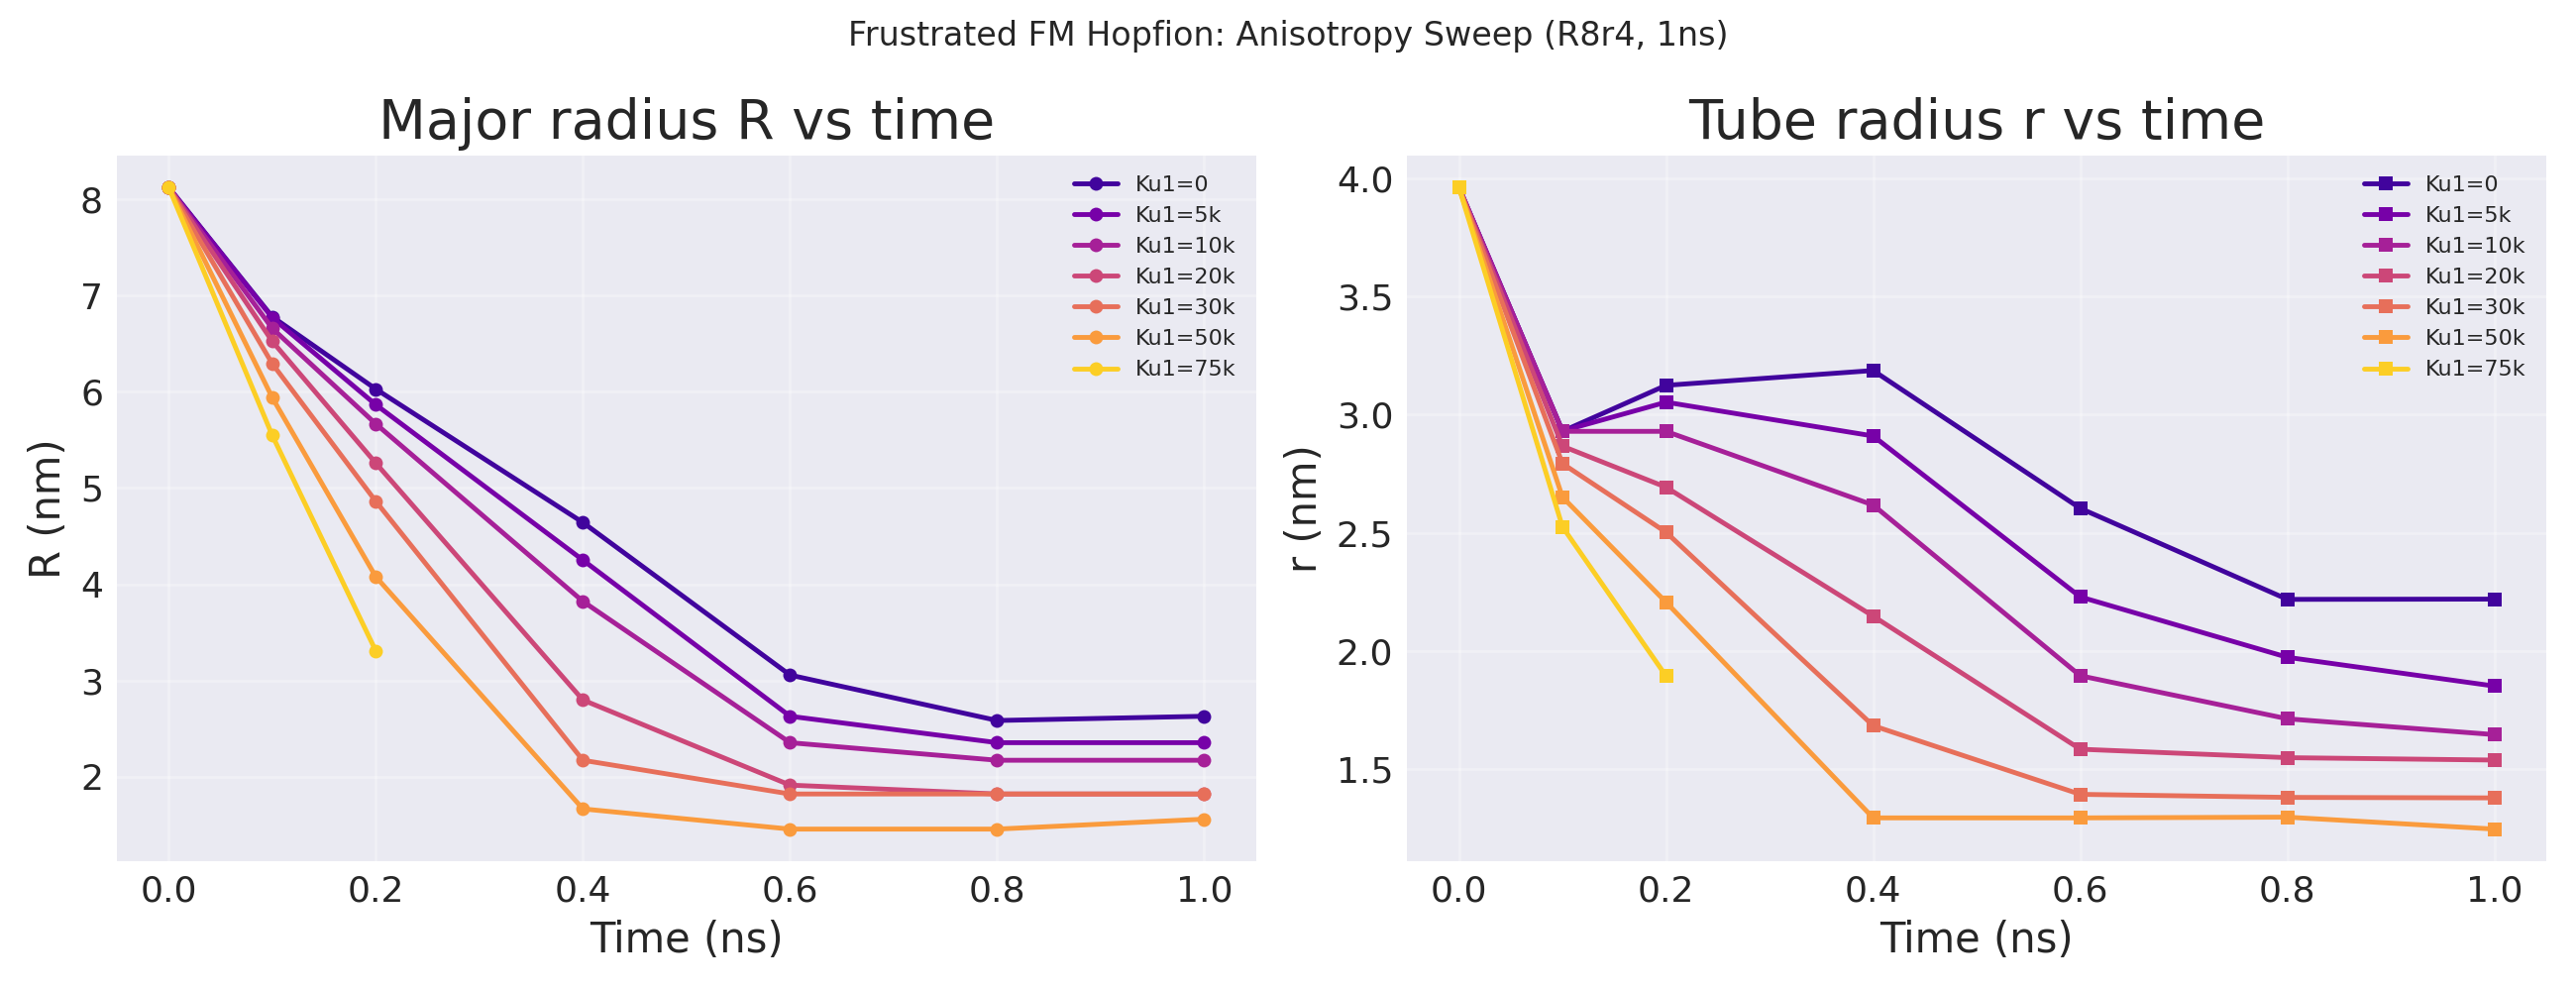
\includegraphics[width=0.95\textwidth]{figures/fig3-6_anisotropy_Rr_vs_time.png}
  \caption{不同 $K_{u1}$ 下 Hopfion 尺寸参数 $R(t)$ 和 $r(t)$ 的时间演化。所有构型从 $R = \SI{8}{nm}$, $r = \SI{4}{nm}$ 出发，$K_{u1}$ 增大导致平衡尺寸持续缩小。$K_{u1} = \SI{75e3}{J/m^3}$ 仅有前 3 帧数据，仿真因 Hopfion 坍缩而中断}
  \label{fig:anisotropy-time}
\end{figure}

\begin{figure}[htbp]
  \centering
  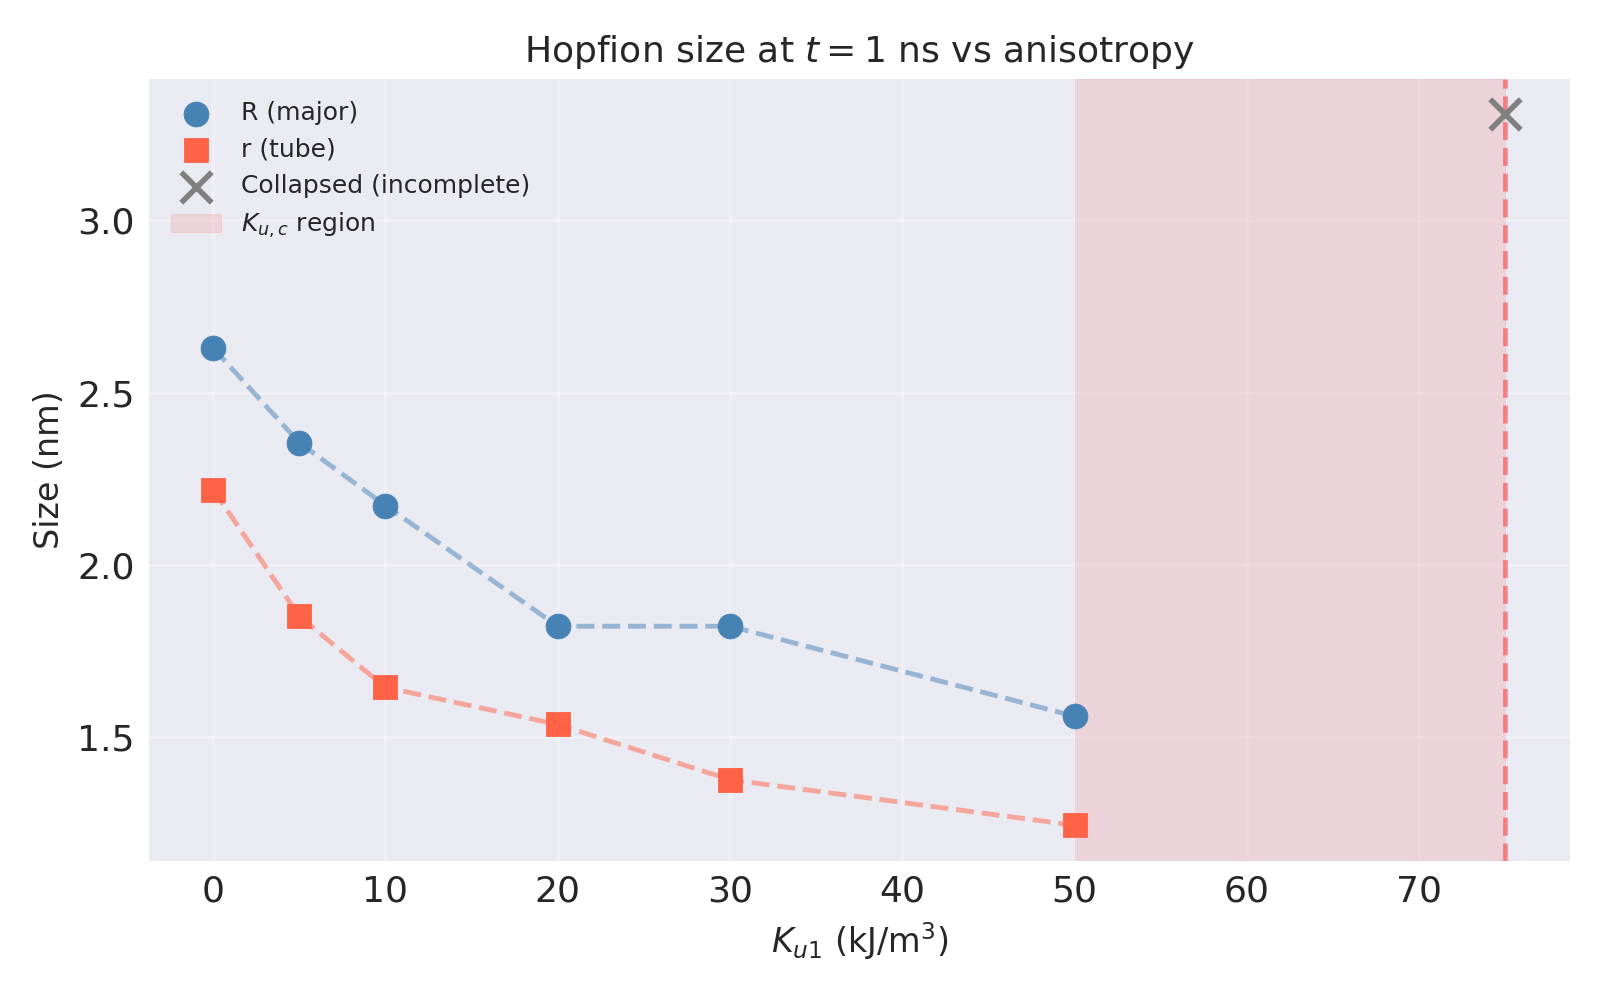
\includegraphics[width=0.8\textwidth]{figures/fig3-7_anisotropy_summary.png}
  \caption{$t = \SI{1}{ns}$ 时 Hopfion 尺寸参数随 $K_{u1}$ 的变化。红色阴影区域标记临界阈值 $K_{u1,c} \in (\num{52e3}, \num{55e3}) \, \si{J/m^3}$，灰色叉号表示 Hopfion 已坍缩}
  \label{fig:anisotropy-summary}
\end{figure}

\subsection{固有尺寸吸引子}

为了研究 Hopfion 弛豫后的平衡尺寸是否依赖初始条件，本文进行了尺寸收敛性测试。本文分别以不同初始尺寸（环面半径 $R$ 和管径 $r$）构造 Hopfion 初始态，在 $\alpha = 5.0$ 的高阻尼下弛豫至稳态，然后用 Python 脚本提取弛豫后的 Hopfion 尺寸。

\cref{fig:size-convergence}展示了尺寸收敛结果。无论初始尺寸如何设定（$R = 3 \sim \SI{12}{nm}$, $r = 2 \sim \SI{5}{nm}$），弛豫后的 Hopfion 均收敛到相同的平衡尺寸：
\begin{equation}
  R_{\text{eq}} = \SI{2.60}{nm}, \quad r_{\text{eq}} = \SI{2.16}{nm}
  \label{eq:attractor}
\end{equation}

这表明该参数下存在一个唯一的\textbf{固有尺寸吸引子}，Hopfion 的平衡尺寸由材料参数唯一确定，与初始条件无关。这也就解释了在配套某一个固定的各向异性参数时，其对应的稳定状态下只会存在一种固定特征的 Hopfion 尺寸。综合各项指标，$K_{u1} = \SI{10e3}{J/m^3}$ 且处于居中位置的 Hopfion 在各项维度均表现最优，因此被选定为后续自旋波驱动仿真（第五章）的初始态。

\begin{figure}[htbp]
  \centering
  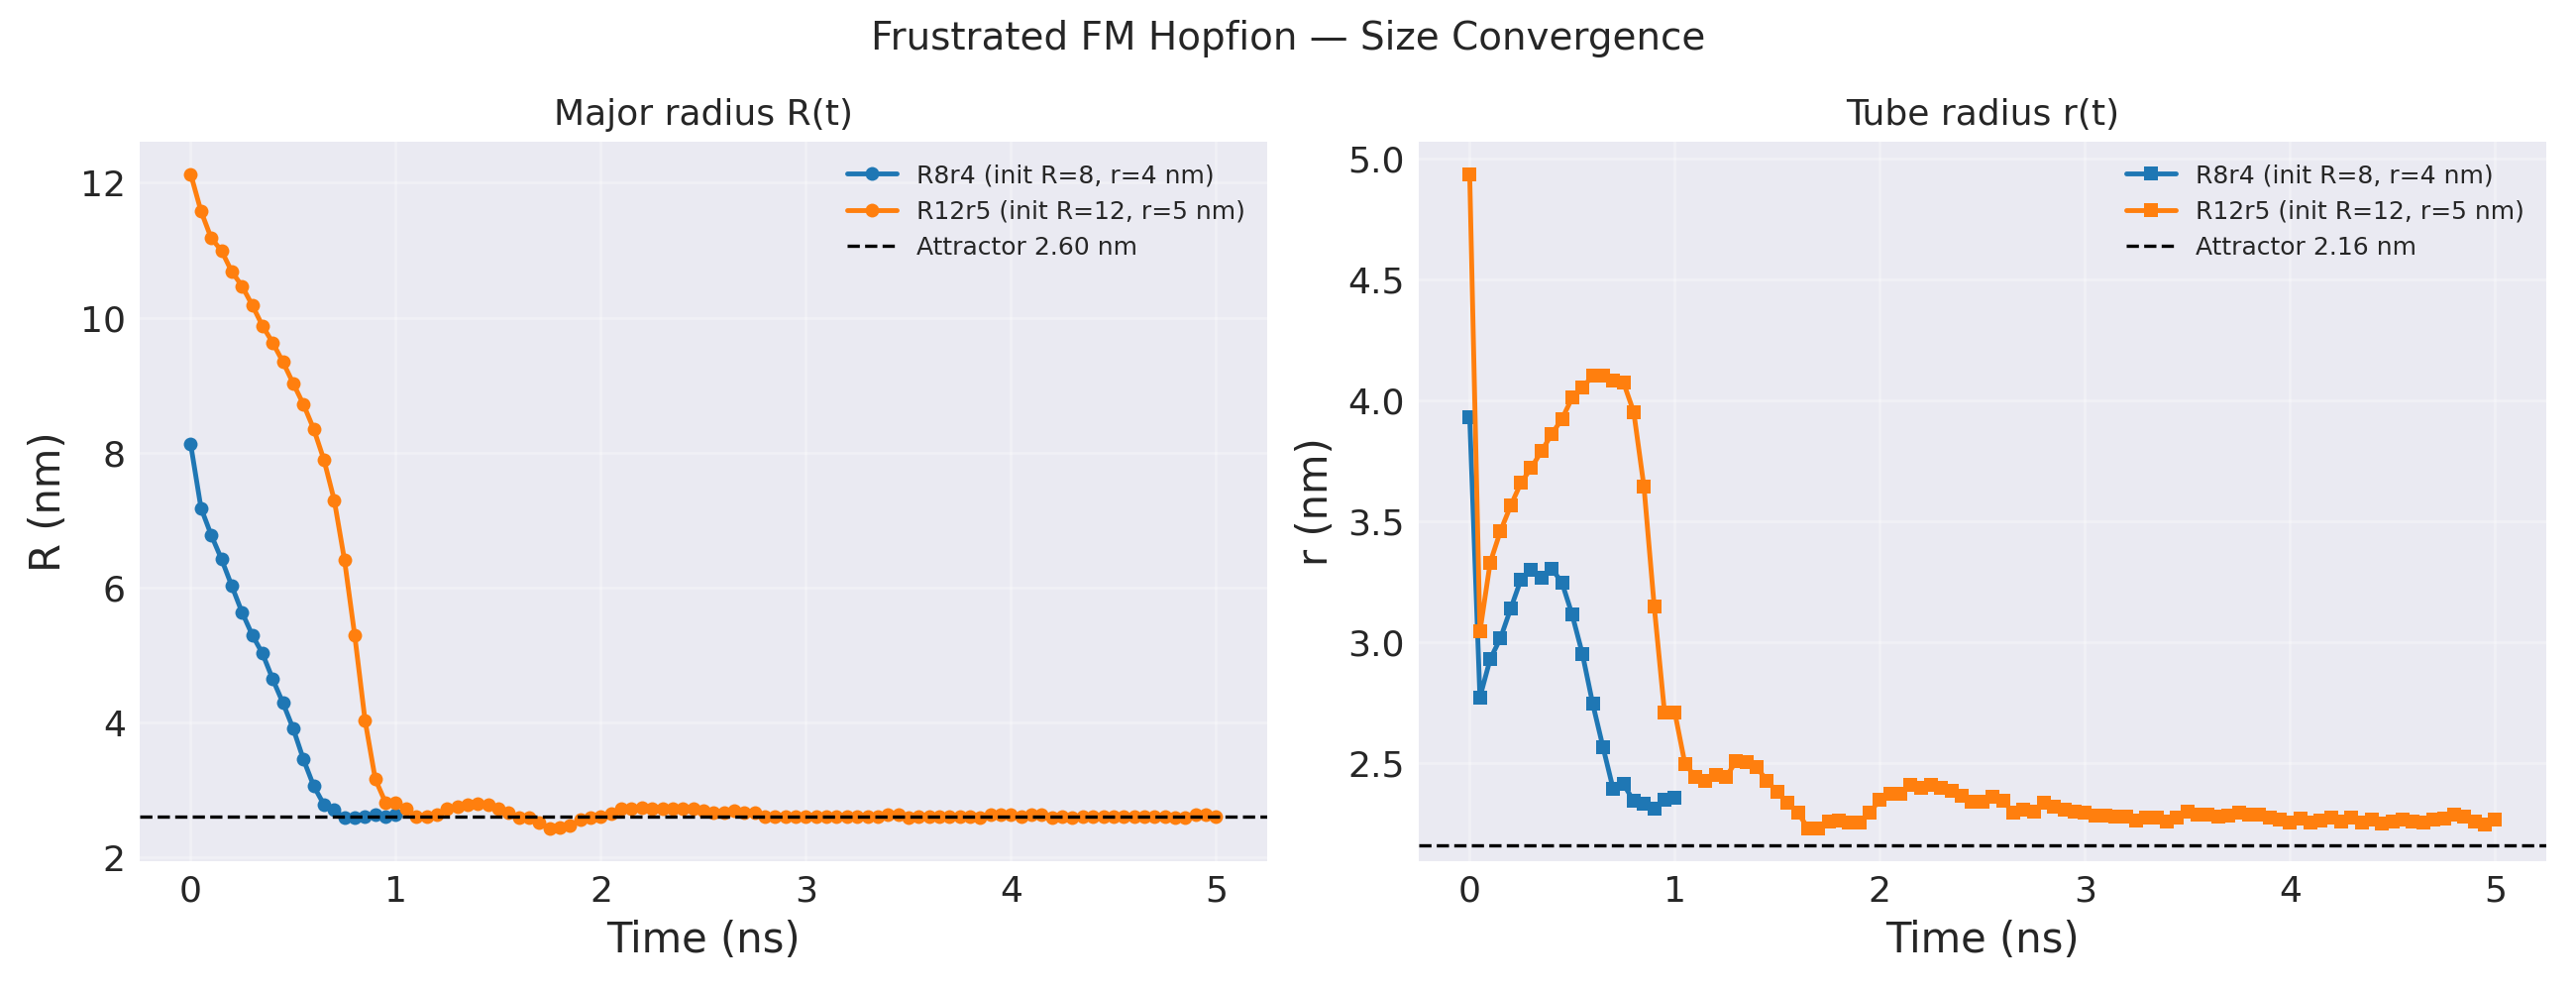
\includegraphics[width=0.95\textwidth]{figures/fig3-3_size_convergence.png}
  \caption{尺寸收敛性测试。不同初始尺寸（$R = 8, \SI{12}{nm}$）的 Hopfion 弛豫后均收敛至相同的平衡尺寸 $R_{\text{eq}} = \SI{2.60}{nm}$, $r_{\text{eq}} = \SI{2.16}{nm}$，证实固有尺寸吸引子的存在}
  \label{fig:size-convergence}
\end{figure}


\section{本章小结}

本章在两种不同的铁磁体系中系统研究了 Hopfion 的稳定条件：

\begin{enumerate}[label=(\arabic*)]
  \item 在 DMI 铁磁（FeGe）体系中，确定了 Hopfion 稳定的三个必要条件：解析初始态构造、边界层冻结、退磁场效应。在 $d = 3\lambda$, $h = \lambda$ 的圆柱模型中实现了 \SI{2}{ns} 稳定。
  \item 在竞争交换铁磁体系中，首先通过控制变量实验证明了背景磁化方向对 Hopfion 漂移行为无影响（四组配置表现完全一致的轴向初始漂移）。
  \item 随后通过周期性平移居中和 \SI{1}{ns} 重新验证，确认了 $m_z$ 背景下居中 Hopfion 的位置稳定性。在此基础上通过细化扫描确定了临界各向异性阈值 $K_{u1,c} \in (\num{52e3}, \num{55e3}) \, \si{J/m^3}$。
  \item 最后验证了固有尺寸吸引子的存在，证明平衡尺寸唯一由材料的各向异性等配套参数确定。综合评估后，$K_{u1} = \SI{10e3}{J/m^3}$ 的居中构型表现最优（$\Delta z = \SI{0.019}{nm}$），被选定为自旋波仿真的初始态。
\end{enumerate}

这些结果是第五章动力学调控研究的基础。第五章的仿真将基于本章确定的稳定参数（$K_{u1} = \SI{10e3}{J/m^3}$、居中构型）进行自旋波驱动实验。
